\documentclass{../local}
\begin{document}
Dit project is gestart vanuit een nieuw concept. Om dit concept mogelijk te maken moet er gebruik gemaakt worden van meerdere componenten. Om een weloverwogen keuze te maken wordt in dit hoofdstuk de keuze gemaakt van de volgende componenten en beargumenteerd waarom die keuze is gemaakt:
\begin{itemize}
\item Keuze van benodigde software aan de hand van de requirements
\item Keuze van hardware die geschikt is voor de gekozen software met in acht neming van de gekozen software

\end{itemize}

\section{Operating System Keuze}
Voor Wireless Sensor Networks zijn vele operating systems (OS) beschikbaar. In deze sectie zullen meerdere met elkaar worden vergeleken en de beste gekozen. Om zeker te zijn dat het mogelijk is om er makkelijk mee te werken, wordt er alleen gekeken naar de populaire OS. Dat betekent dat het OS programmeer voorbeelden moet hebben, in het laatste jaar aan moet zijn ontwikkeld en het bekend is dat er door andere partijen actief gebruik van wordt gemaakt.

\begin{wrapfigure}[15]{r}{0.55\textwidth}
	\vspace{-20pt}
	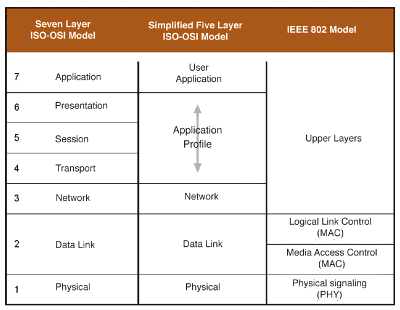
\includegraphics[width=9cm]{../images/OSI-IEE802}
	\caption{\emph{OSI model IEEE 802.15.4 \cite{gutierrez2004low}}} \label{fig:OSIIEEE}

\end{wrapfigure}

De volgende OS'en of oplossingen worden bestudeerd: ZigBee, Z-Wave, TinyOS, ContikiOS en RIOT. Voor elk onderdeel wordt beschreven hoe het systeem werkt en daarna de voordelen en nadelen uiteen gezet.

\subsection{ZigBee}

ZigBee is een standaard bedoeld voor low-cost, energiezuinige draadloze 'mesh'- of 'ster' netwerken. Een mesh netwerk maakt het mogelijk om een hoge robuustheid te garanderen en groot netwerk op te bouwen. Deze netwerken kunnen theoretisch tot ongeveer 65.000 nodes bestaan. Zigbee huisvest ook routing technieken en beveiliging binnen de netwerken. Ontwikkelaars die ZigBee gebruiken of de ZigBee standaard verbeteren zitten binnen de ZigBee Alliance, wel te vergelijken als de WiFi Alliance.

Een zigbee netwerk bestaat uit 3 componenten: één ZigBee Coordinator, ZigBee Routers en ZigBee End Devices. De Coordinator is de maker van het netwerk en bepaalt de netwerk instellingen en beveiliging. Routers zijn bedoeld om het netwerk te vergroten en berichten door te sturen. End Devices zijn randapparaten die de omgeving meten of controleren.

ZigBee is gebouwd op de IEEE standaard 802.15.4. Deze standaard beschrijft de fysieke laag en de data-link laag van het OSI model te zien in in de rechter kolom van figuur \ref{fig:OSIIEEE}. De fysieke laag van het OSI model bepaalt hoe data draadloos wordt verzonden (modulering) en in welke radioband. De Data-Link laag beschrijft controle mechanismes hoe en wanneer een module binnen een IEEE 802.15.4 netwerk mag verzenden. De overdrachtsnelheid hierbij is 250 kb/s bij gebruik van het 2.4GHz spectrum wat wereldwijd beschikbaar is.

De opvolgende lagen van het OSI model zijn ingevuld door de ZigBee standaard. ZigBee volgt het versimpelde vijf lagen OSI model te zien in figuur \ref{fig:OSIIEEE}. ZigBee biedt applicatie profielen aan die functionaliteiten bieden voor bepaalde gebieden zoals: Home Automation, Snart Energy of Building Automation. Bovenop deze profielen kan de benodigde applicatie gebouwd worden.\footnote{\url{http://www.zigbee.org/}}

\subsubsection{Voordelen/Nadelen}

ZigBee is veelgebruikt en er zijn vele bedrijven die oplossingen aanbieden. Ook zijn er veel programmeer voorbeelden beschikbaar via verschillende leveranciers zoals Texes Instruments en Libelium. Het gebruik van de Zigbee profielen versimpelt de ontwikkeling van applicaties aanzienlijk.

Bekend met ZigBee is dat het netwerk gedeelte onveranderbaar is. Er kan een netwerk topologie gekozen worden waar dan niet van kan worden afgeweken. Wel alle belangrijke soorten topologieën zijn beschikbaar.

Het netwerk van ZigBee werkt met een centrale Coordinator die zaken als routing en veiligheid verzorgen. In de oudere ZigBee standaard (2006) resulteerde het falen van de coordinator tot het falen van het netwerk. Dit is in nieuwere versies opgelost door de optie te bieden om binding tables van een netwerk te distribueren over het gehele netwerk.

Hoewel dit een verbetering is, geeft het niet de flexibiliteit en robuustheid voor End Devices. End Devices die als nieuw of opnieuw het netwerk moeten betreden of kunnen dat niet meer wanneer de coordinator is uitgevallen. Dit is niet praktisch bij een veiligheidsinstallatie voor branddetectie. Nodes (of Devices in het geval van ZigBee) binnen een netwerk kunnen bij brand of andere situatie uitvallen. Een ZigBee netwerk kan hiermee slecht omgaan.

%ik bedoel hier dat de specificaties van zigbee niet zomaar beschikbaar zijn...
Het is ook niet mogelijk om de netwerklaag van ZigBee aan te passen gezien het type licentie wat er aan gekoppeld zit. Verkoop van producten die ZigBee gebruiken moeten overigens ook lid zijn van de ZigBee Alliance, wat op moment van schrijven vanaf \$4.000 per jaar kost\footnote{\url{http://www.zigbee.org/Join/MembershipForms.aspx}}.

\subsection{Z-Wave}
Z-Wave is een gepattenteerde draadloze standaard ontwikkeld door Zensys en eigendom van Sigma Designs.
\subsection{TinyOS}
%lang vooruitstaand OS. veel support
% - nieuwe programmeertaal NESC

% + 6LoWPAN

\subsection{ContikiOS}
%vrije RIME protocol. compatible met 802.15.4 frames
%simpele driver development
%switchen van mac protocol / RDC protocol
%maken van dit soort dingen is relatief simpel( mac / rdc ).
%++++++SIMULATIE
\subsection{RIOT}
%nieuw/vers, weinig platformen


Aan de hand van de requirements kan de keuze van de techniek verschillen. Energiebehoefte, bandbreedte en bereik zijn van invloed op de keuze. In deze sectie zal de gekozen oplossing worden beschreven en beargumenteerd.

Wireless sensor netwerken zijn volgens de volgende punten te karakteriseren: beperkte performance, mobiel, goedkoop te produceren en lage bandbreedte eisen \cite{akyildiz2002wireless}.


%Bij het gebruik van een draadloze verbinding wordt standaard gedacht aan een WLAN ( wireless local area network ) verbinding. In het kader van WSN's is een WLAN verbinding niet toereikbaar aangezien een WLAN verbinding vele relatief complexe requirements met zich meebrengt (lange afstanden overbruggen, hoge bandbreedte). Dit resulteert direct in duurdere hardware die veel stroom nodig hebben om de requirements te behalen. De complexiteit van een dergelijke standaard geeft ook extra restricties met zich mee, zoals het nodig hebben van genoeg opslagruimte voor de programma-code.

%Het concept WPAN ( Wireless Personal Area Network ) is ontworpen om deze eigenschappen om te gooien. Dit concept maakt het mogelijk om goedkope en energie efficiënte netwerken op te zetten. Dit soort netwerk is van toepassing op dit project.

%dit verwijderen?
Gebouwd op het WPAN concept een IEEE standaard ontwikkeld die WSN's mogelijk maakt. De IEEE standaard 802.15.4 beschrijft een standaard die de bovengenoemde karakteristieken huisvest. Deze standaard beschrijft ook een energiebeheersysteem om het verbruik zo laag mogelijk te houden. Deze klasse wordt als LR-WPAN geclassificeerd (Low Rate WPAN). In figuur 4.1 is te zien hoe deze drie soorten netwerk types tegenover elkaar staan.


De vastgestelde IEEE 802.15.4 standaard beschrijft naast de fysieke requirements ook netwerk topologieën. De standaard definieert dat een netwerk in een ster- of een peer-to-peer topologie opereert. De onderdelen binnen een dergelijk netwerk kan 2 soorten apparaten bevatten, een 'coordinator' of een reguliere 'device'. Een Coordinator binnen een netwerk is de initialisator binnen een netwerk waarbij de devices de onderdelen hiervan zijn. Binnen een ster netwerk zal voornamelijk één device horen bij één coordinator, waarbij één coordiantor met meerdere coordinatoren of devices kan communiceren.

Wanneer wordt gesproken over datacommunicatie, wordt het OSI model ook meegenomen. De standaard hierboven beschreven staat alleen voor de onderste twee lagen van het OSI model; De fysieke laag en de data link laag. De lagen daarboven zijn niet gespecificeerd. wanner deze bovenste lagen worden gespecificeerd, moet rekening gehouden worden met de grenzen van de hardware binnen een WSN, die erg gelimiteerd zijn aan processorkracht of RAM geheugen.
\\\cite{gutierrez2004low}

Zoals hierboven beschreven is het gebruik van de IEEE standaard 802.15.4 vanzelfsprekend bij gebruik van een WSN. Dit is dan ook de keuze als draadloze transmissie techniek voor dit project. Deze techniek kan opereren in een van de drie radio frequentie banden:
\begin{itemize}
\item 868.0–868.6 MHz. (drie kanalen) Alleen in Europa beschikbaar
\item 902-928 MHz. (dertig kanalen) Alleen in Noord Amerika beschikbaar
\item 2400-2483.5 MHz. (zestien kanalen) Wereldwijd beschikbaar.
\end{itemize}

\section{Software}
Zoals aangegeven in de vorige sectie en Figuur 4.2 is de keuze van een draadloze transmissie standaard nog niet alles. Er moet nog extra software komen om de volgende lagen van het OSI model op te vullen. Beschikbare oplossingen zijn: Zigbee, 6LoWPAN en RIME.

\section{Hardware}
Met gebruik van de gekozen wireless transmissie techniek, software en de requirements kan de hardware gekozen worden. 
%

\end{document}